\documentclass[11pt]{article}
\usepackage{icmlko}
\begin{document}

\title{만화가 처음으로 채점된다 --- 인기순 수집이 잘라 놨던 258행}
\author{월드모델 실험실}
\date{노트 370 · 2026년 8월 1일}
\maketitle

\begin{abstract}
노트 356부터 여덟 편이 만화 하나를 쫓았다. \textbf{끝났다.} 만화가 유보
258행으로 \textbf{열한 번째 채점 도메인}이 됐다 --- $\rho = 0.2520$,
95\% $[0.127,\,0.350]$, 폭 0.223 으로 \textbf{판에서 셋째로 좁은 구간}이다
(웹툰 · 애니 · 모바일 다음). 판은 $0.4862 \to 0.4654$ 로 내려가고 분모가
$2{,}723 \to 2{,}981$ 로 바뀌어 옛 수와 직접 못 견준다. \textbf{대신 순서를
못 가리는 쌍이 67\%(30/45)에서 60\%(33/55)로 준다.}

가는 길에 두 가지를 채택했다. ① \textbf{채움을 재현 가능하게}
(\texttt{ingest/media\_push.py}) --- 짝으로 재면 옛 채움과 $-0.0011$
(SD 0.0021, 5/12)로 사실상 같은데, 옛 것은 \emph{만든 스크립트가 없어
새 행에 못 쓴다}. 노트 367이 방금 적은 ``자료 결정은 재현 가능해야
한다''가 여기서 갈랐다 --- 점수가 아니라. ② \textbf{만화 258행}.
\textbf{둘 다 점수를 내린다} --- 그것이 점수를 보고 고른 게 아니라는
검산이다(노트 353 · 354 · 365와 같은 방향).
\end{abstract}

\section{여덟 편이 쫓은 것}

\begin{center}
\begin{tabular}{ll}
\hline
노트 & 무엇을 알았나 \\
\hline
356 & 만화는 학습 1,783행(17\%)인데 한 번도 채점이 안 된다. 빼면 판이 오른다 \\
361 & 희석이 아니다 --- 절반을 빼면 0 \\
362 & \textbf{문턱}이다 --- 178행은 0행과 같고 892행은 1,783행과 같다 \\
363 & 복도 위험은 만화가 11위다. 예상이 깨졌다 \\
364 & 남에게 주는 해는 세계애니와 \textbf{같다}($+0.003$). 다른 건 \emph{값을 치르느냐} \\
365 & 유보 6행은 자료가 없어서가 아니라 \textbf{인기순 수집}이 잘랐다 \\
366 & 우회로(축 끄기) 막힘. 그리고 미결정 폭이 낡았다 \\
368 & 채움을 다시 만드니 개념은 맞는데($+0.9905$) 눈금이 틀렸다 \\
369 & 옛 채움 $=$ \textbf{제 도메인 백분위}. 복원 완료 \\
\textbf{370} & \textbf{넣는다} \\
\hline
\end{tabular}
\end{center}

\section{두 가지를 채택한다}

\begin{center}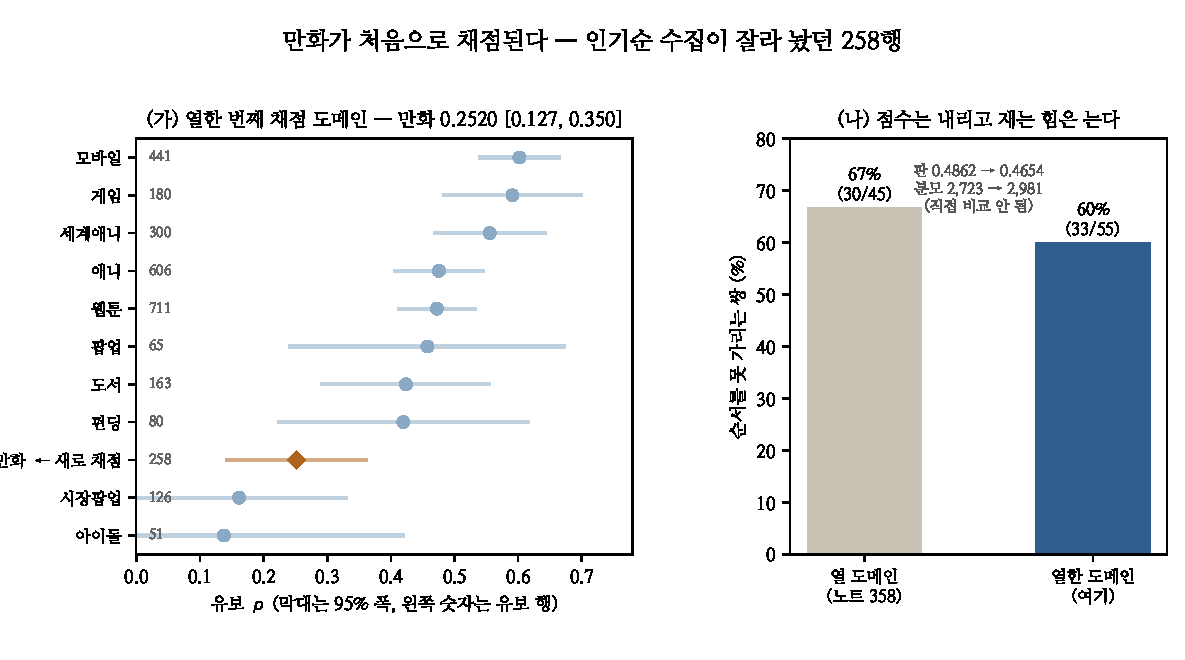
\includegraphics[width=\linewidth]{figs/eleventh.pdf}\end{center}

\textbf{① 채움 재현}(\texttt{ingest/media\_push.py}). 짝 열둘로 재니
판 $-0.0011$(SD 0.0021, \textbf{5/12}) --- 노트 367 규약으로 미결정이고
배포(팝업 $+0.0031$, 8/12)도 못 정한다. \textbf{점수로는 무승부다.}
갈라 준 것은 다른 조항이다:

\begin{quote}
\textbf{자료 결정은 재현 가능해야 한다}(노트 367).
\end{quote}

옛 채움은 만든 스크립트가 없어 \emph{새 행에 값을 줄 수 없다}. 새 것은
\texttt{data/state/manga\_links.json} $\cdot$
\texttt{wanime\_links.json} 에서 여덟 줄로 다시 만들어진다. \textbf{같은
값이면 재현되는 쪽을 쓴다} --- 그리고 이 조항은 결과를 보기 전에 적혔다.

\textbf{② 만화 258행.} 노트 365가 긁어 놓고 노트 368 · 369가 채움을
복원할 때까지 못 넣던 것이다.

\begin{center}
\begin{tabular}{lrr}
\hline
 & 전(노트 358) & 지금 \\
\hline
채점 도메인 & 10 & \textbf{11} \\
만화 유보 & --- (6, 문턱 아래) & \textbf{258} \\
만화 $\rho$ & --- & $0.2520\,[0.127,\,0.350]$ \\
판 & 0.4862 & 0.4654 \\
판 분모 & 2,723 & 2,981 \\
판 95\% & $[0.4534,\,0.5162]$ & $[0.4312,\,0.4924]$ \\
\textbf{못 가리는 쌍} & 30/45 (67\%) & \textbf{33/55 (60\%)} \\
\hline
\end{tabular}
\end{center}

\textbf{만화 구간 폭 0.223 은 판에서 셋째로 좁다} --- 웹툰(0.127) ·
애니(0.147) · 모바일(0.128) 다음이고 게임 · 세계애니보다 좁다. 유보
258행이 그만큼 한다. \textbf{노트 352가 ``45쌍 중 30쌍을 못 가린다''로
연 갈래가 처음으로 좋아졌다.}

\section{회계가 닫혔다}

노트 364가 정리한 것: 만화는 남에게 $+0.0035$ 를 물리면서 제 점수가
없어 아무 값도 안 냈다. 세계애니는 같은 해를 끼치지만 제 300행을 맞혀
판의 11\%를 벌어 온다. \textbf{만화의 빈칸이 채워졌다} --- 이제 258행 ·
가중 8.7\% 를 벌어 온다(그 값이 $0.2520$ 으로 낮을 뿐이다).

\textbf{그래서 판이 내려간 것은 나빠진 것이 아니다.} 원래 치르고 있던
값이 이제 장부에 적힌다. 노트 361이 ``남은 것 표의 수는 인용할 때마다
다시 잰다''고 적은 것과 같은 자리다 --- \emph{안 재던 것을 재기 시작하면
수는 내려간다.}

\section{읽을 때 조심할 것}

\textbf{만화 유보는 학습과 다른 모집단이다.} 학습 1,783행은 인기 상위
2,000건 훑기에서 왔고, 유보 258행은 시작일 2025년 이후 전부다(유보 라벨
중앙 1,133 대 2023\textasciitilde{}24 학습 8,226). \textbf{유명한 만화로 배워
신작 전부를 맞히는 과제}이고, 그것이 더 옳은 과제이지만 \emph{다른}
과제다. 노트 284가 시장팝업에 붙인 주의와 같은 종류다.

시계는 재 봤다 --- 학습 $-0.159$ · 유보 $-0.202$ · 달력 기준선 0.202 대
모형 0.2520 이다. 노트 270의 눈금으로 시계 몫이 \textbf{0.80} 이라
도서(1.52)보다 낫지만 웹툰(0.77) 수준으로 높다. \textbf{만화만 오르는
결과는 믿지 않는다.}

\section{남은 것}

\begin{center}
\begin{tabular}{ll}
\hline
갈래 & 지금 아는 것 \\
\hline
만화 KR/CN 583행 & 노트 79가 근거를 대고 뺐다. 지금 판에서 다시 재나 \\
세계애니 눈금 & 합친 백분위가 세계애니를 12/12 로 올렸다(노트 369) \\
팝업 실측 41행 & 노트 360 · 364 · 366. 결정 다섯을 팝업이 내렸다 \\
아이돌 0.1375 & 이번 창에서 계속 내려왔다(0.4860 → 0.1375). 왜 \\
\hline
\end{tabular}
\end{center}

마지막 줄이 새로 보인다 --- 아이돌은 노트 353에서 유보를 51로 늘린 뒤
계속 내려왔고, 지금은 판에서 제일 낮다. 유보 51행이라 구간이 넓지만
방향이 한결같다.

\end{document}
